\section{Pol-Nullstellenplot}

In Abbildung \ref{fig:pnp} ist der Pol-Nullstellenplot des Systems zu sehen.\\ Die mit x markierten Stellen zeigen die beiden Polstellen an. Dieses System hat keine Nullstellen und ist somit kausal, da es mindestens so viele Polstellen wie Nullstellen besitzt.\\  Die Polstellen des Systems befinden sich im negativen (0 inkludiert) Teil der reell-wertigen Achse und liegen somit in der linken Halbebene.\\ \\
Die Polstellen entsprechen den Eigenwerte der Systemmatrix $A$:
\begin{eqnarray*}
A = \begin{bmatrix} 0 & 1 \\ 0 & -\frac{1}{7}\end{bmatrix} \\
\lambda_1 =  0 \qquad \Re(\lambda_1) &=& 0 \\ \lambda_2 = -\frac{1}{7} \qquad \Re(\lambda_2) &=& -\frac{1}{7} < 0
\end{eqnarray*}


$\Rightarrow$Das System ist stabil.

\begin{figure}[H]
	\centering
	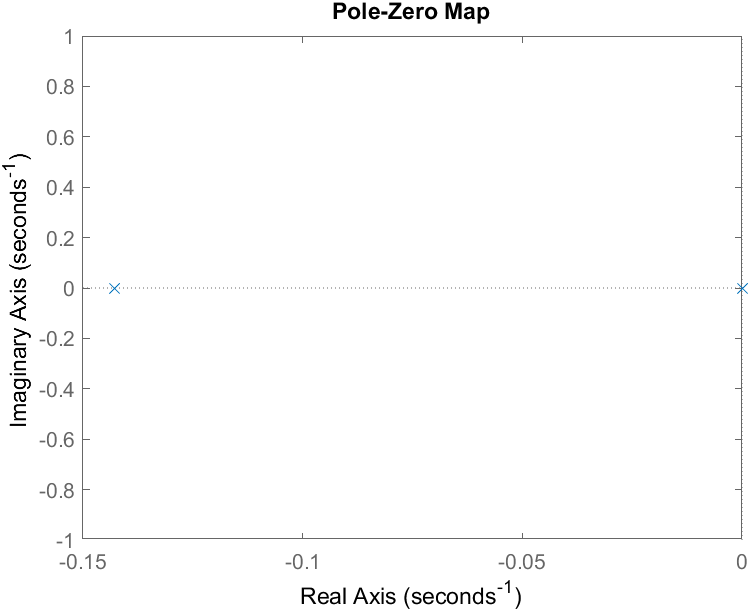
\includegraphics[width=0.8\textwidth]{{diagrams/pol_nullstellenplot.png}}
	\caption[Pol-Nullstellenplot]{Pol-Nullstellenplot}
	\label{fig:pnp}
\end{figure}